\documentclass{report}

%------------- Préambule --------------
\usepackage[utf8]{inputenc}
\usepackage[francais]{babel}
\usepackage[T1]{fontenc}

\usepackage{graphicx} % Pour les figure
\graphicspath{{images/}} % Toutes les images se trouvent dans le dossier images
\usepackage{float}
\usepackage[T1]{tipa} % Pour la phonétique
\usepackage[francais]{minitoc} % Pour les mini sommaires


\setcounter{tocdepth}{-1}
\setcounter{parttocdepth}{2}


\usepackage[colorlinks=true]{hyperref} 
\hypersetup{urlcolor=blue,linkcolor=black,citecolor=black,colorlinks=true}


%------------- Corps --------------
\begin{document}
	\doparttoc % Pour les mini sommaires dans les parties
	
	
	%------------------------------------------------- Page de garde -------------------------------------------------%
	%------------------------------------------------- Page de garde -------------------------------------------------%
\begin{titlepage} 
	\begin{center}
		\Huge{\textbf{Dimension Commerciale}}\\
		\vspace{0,5cm}
		\large {Doriane \bsc{Peresse}, Maxime \bsc{Catoire}}\\
		\vspace{0,5cm}
		\large {HES - \today}
	
		\vfill 

		\huge{Dans quelle mesure l'amélioration de la plateforme par notre projet peut-elle donner à l'entreprise l'opportunité d'étendre la distribution de son produit ?}

		\vfill 
	
	\end{center}
\end{titlepage}	
	
	
	
	
	%------------------------------------------------- Début du document -------------------------------------------------%
	\tableofcontents
	
	
	%---------------------------------------------------- I. Introduction ---------------------------------------------------%
	
	%---------------------------------------- Introduction ----------------------------------------%


	
	\section{Introduction}
	Ce projet transversal est issu de la collaboration de l'Ecole Polytechnique de l'Université de Nantes et de l'entreprise Project2Cloud. Il sera mené de bout en bout par deux étudiants de quatrième année du cycle ingénieur du département informatique, supervisés par deux professeurs référents. Il s'étendra de septembre à mai. L'objectif est de permettre aux étudiants en charge de réaliser un projet professionnel dans le cadre de leurs études. Au delà de la dimension technique, les projets informatiques intègres des notions plus larges et plus actuelles. Il est donc important de prendre conscience que les projets transversaux présentent des enjeux organisationnels, marketing et/ou écologiques. Il conviendra de faire une étude d'une de ces trois dimensions, en s'appuyant sur les enseignements dispensés dans le module Homme Entreprise et Société. 
	
	Nous commencerons par présenter l'entreprise et son produit, puis nous détaillerons le projet qui nous a été proposé. Nous continuerons en présentant la problématique marketing que nous avons décidé de développer, ainsi que l'explication du choix de cette dimension. Enfin, nous ferons l'étude marketing de ce projet, et terminerons pas une conclusion qui synthétisera notre étude. 
	
	
	%------------------------------------------------- II. Contexte du projet ------------------------------------------------%
	
		%------------------------------------------------- Contexte du projet ------------------------------------------------%

	\part{Contexte du projet}
	
	\setcounter{chapter}{1} % Pour recommencer la numérotation des chapitres à 1
	\setcounter{section}{0} % Pour recommencer la numérotation des section à 1
	
	\section{L'entreprise : Project2Cloud}
	Project2Cloud est une plate-forme de gestion collaborative. Une site de présentation est déjà en ligne à l'adresse http://project2cloud.org/. Elle propose différents services de communication, tels que la vidéo-conférence, le chat et la conversation audio. Le but est d'offrir aux utilisateurs un panel complet de communication, leur permettant d'échanger en temps réel des informations et des services. Project2Cloud innove également avec la possibilité d'associer aux sessions de dialogue des documents de différents types (texte, vidéos...). Le document associé à la session permet de créer une "mémoire" numérique du document, autour de laquelle de nouvelles connaissances peuvent venir s'ajouter à tout moment.
	
	P2C (abréviation courante de Project2Cloud) est géré par trois informaticiens passionnés depuis maintenant 1 an. La plate-forme P2C est pour le moment en béta-test privé, c'est à dire qu'elle n'est pas encore accessible. Elle est actuellement testée par plusieurs industriels. Pour les besoins du projet, un accès nous a été donné à la version opérationnelle de la plate-forme. Cette version nous permet d'avoir une idée de l'application qui sera prochainement disponible.
	
	\section{Notre projet : Transcriptions audio vers texte pour des réunions enregistrées}
	Notre projet s'implantera directement dans la plate-forme P2C. Comme nous l'avons expliqué précédemment, P2C permettra aux utilisateurs de communiquer facilement grâce à un panel complet d'échanges vidéo, audio ou texte. Le but de notre projet est de faciliter l'indexation des conférences vidéos (c'est à dire de mieux séquencer temporellement les vidéos enregistrées). Pour cela, nous devrons ajouter une fonctionnalité supplémentaire : la transcription vocale des conversations. Concrètement, lors d'une conférence vidéo, les conversations des différents participants seront traduites en texte. Ce même texte sera enregistré sur un serveur. Le but est de permettre à un utilisateur de retrouver un mot ou un groupe de mot prononcé pendant une conférence, et de pouvoir visionner cette dernière à l'instant où le mot a été prononcé. On créé ainsi une "mémoire" des conférences, avec la possibilité de retrouver des informations très précises à des moments clés. 
	Notre projet est donc de convertir les conversations en texte, de les enregistrer, et de pouvoir indexer ces conversations à partir de mots clés.
	
	
	%------------------------------------------------- III. Cahier des charges ------------------------------------------------%
	
		%------------------------------------------------- Cahier des charges ------------------------------------------------%

	\part{Cahier des charges}
	\parttoc
	
	
	\setcounter{chapter}{0} % Pour recommencer la numérotation des chapitres à 1
	\setcounter{section}{0} % Pour recommencer la numérotation des section à 1
	
	\chapter{Fondements du projet}

		\section{Contexte du projet}
		Le projet proposé est le fruit de la collaboration de l'école polytechnique de l'université de Nantes et de l'entreprise Project2Cloud. Il sera mené de bout en bout par deux étudiants de quatrième année du cycle ingénieur, supervisés par deux professeurs référents. Il s'étendra de septembre à mai. 

		\section{Objectifs du projet}
		L'objectif est de permettre aux étudiants en charge de réaliser un projet professionnel dans le cadre de leurs études. L'objectif du projet est d'ajouter à une plateforme de communication existante un module de transcription textuelle. Chacune des vidéos enregistrées sur la plateforme aura donc un fichier texte associé, qui correspondra à la transcription textuelle de l'audio de cette vidéo. L'intérêt est de rendre plus facile la recherche d'informations à travers les archives vidéos des réunions passées. 

	\chapter{Personnes et organismes impliqués dans le projet}
		\section{Maître d'ouvrage}
		Le maître d'ouvrage sera le contact principal de l'entreprise. C'est avec lui que les étudiants et les tuteurs enseignants seront en relation. Il devra constamment être informé de l'avancement du projet ainsi que des difficultés éventuelles rencontrées. Il pourra interférer à tout moment dans le projet. Son rôle sera de s'assurer que le projet se déroule comme il le désire. Il pourra au besoin demander des modifications ou apporter des précisions sur des points non spécifiés. Toutes les modifications apportées au projet en cours devront être discutées avec les élèves et tuteurs enseignants, pour s'assurer que les objectifs restent adaptés aux contraintes pédagogiques des projets transversaux.  

		\section{Tuteurs enseignants}
		Le rôle des tuteurs enseignant est d'encadrer les étudiants tout au long du projet. Ils devront être tenus informés chaque semaine de l'avancement du projet, ainsi que des difficultés rencontrées. Les tuteurs auront pour rôle de guider les étudiants dans la démarche organisationnelle du projet, et de s'assurer que les objectifs fixés sont respectés à la fin de chaque phase de travail.

		\section{Elèves Étudiants}
		Les deux étudiants seront les concepteurs du projet. C'est à eux de mener de bout en bout le projet. Avec l'aide des tuteurs enseignants et du maître d'ouvrage, ils devront mener à bien le projet, de sa phase de recherche à sa phase de conception. Ils devront rendre compte de leur travail chaque semaine, et respecter les différentes contraintes imposées par le cahier des charges (contraintes temporelles, technologiques...). 

		\section{Utilisateurs du produit}
		Les utilisateurs seront les usagers de la plateforme Project2Cloud. Le projet sera ainsi destiné aux personnes ayant créées un compte sur la plateforme, et désirant rechercher une vidéo. En effet, lors de la recherche vidéo, ce sont les fichiers de transcription associés aux vidéos qui seront utilisés. 


	\chapter{Contraintes sur le projet}

		\section{Contraintes négociables}
			\subsection{Types de modules externes utilisés}	
			L'utilisation de modules et logiciels \bsc{libres} est recommandé. Cette mesure est fonction de la quantité et de la qualité des modules accessibles. Dans le cas où les solutions libres ne correspondraient pas aux attentes du client, l'utilisation de modules propriétaires sera envisagée. Une discussion avec les tuteurs et le maître d'ouvrage devra alors être tenue pour trouver le meilleur compromis technique et financier. 

			\subsection{Environnement de développement du projet}
			\subsubsection{Système d'exploitation}
   			Le projet sera développé pour être utilisé sur une plateforme Linux. 

			\subsubsection{Logiciel et langage de programmation}
			 Le langage informatique utilisé est le langage de programmation orienté objet Java, puisque la plateforme déjà existante est elle même codée avec ce langage. 

			\subsection{Langage reconnu par les modules de transcription}
			Le projet développé sera principalement axé sur la langue française. Le module de transcription devrait donc reconnaître des conversations françaises. Dans le cas où les modules français ne seraient pas suffisamment performant ou indisponibles, une solution de traitement en Anglais pourrait être envisagée. Il conviendrait dans ce cas de discuter avec le maître d'ouvrage et les tuteurs enseignants de la suite à donner au projet. Les recherches d'un module français pourront être abandonnées ou se poursuivre tout au long du projet, dans le cas où un nouveau module serait disponible. 

			\subsection{Fonctionnalités supplémentaires}
			Des fonctionnalités supplémentaires pourront être ajoutées en cours du projet. Ces ajouts éventuels seront fonction de l'avancement du projet, de la validation des fonctionnalités prioritaires. Le choix des fonctionnalités supplémentaires sera discuté avec le maître d'ouvrage et les tuteurs enseignants, pour s'assurer que ces nouveautés restent en accord avec la portée pédagogique du projet transversal. 

		\section{Contraintes non négociables}
			\subsection{Contraintes de temps}				
		Le projet débute après la réunion de lancement qui s'est tenue le 30 septembre 2011, en présence du maître d'ouvrage, des tuteurs et des élèves. Il devra être mené à terme avant le 26 mai 2012. Les étudiants auront à leur disposition une demie-journée par semaine réservée à la mise en œuvre du projet transversal.  
				

		        \subsection{Environnement de fonctionnement du projet}
			La plateforme de communication est actuellement fonctionnelle. Elle est accessible sur internet, via tous les navigateurs web et tous les systèmes d'exploitation(MaC, Windows, Linux). 

			\subsection{Lieu de fonctionnement}
			La plateforme de communication sur laquelle repose le projet est utilisable depuis n'importe quel type d'ordinateur(PC fixe, portable). Par conséquent, et au vue de la mobilité des supports, la plateforme peut être utilisée dans des environnements variés (salle de réunion, lieu public, environnement extérieur...). La contrainte sonore est capitale dans notre projet. Un son ambiant relativement restreint, voir faible est essentiel pour une utilisation optimale du projet.   
	

			\subsection{Contraintes matérielles}
			L'utilisation du produit se fera par l'intermédiaire d'un micro. Il pourra s'agir de différents types de micro (micro intégré à l'ordinateur, micro externe). De la qualité du micro dépendra la qualité de la transcription. En cas de besoin matériel spécifique au projet, l'entreprise devra être en mesure de le fournir. 

			\subsection{Quel est le budget affecté au projet ?}
			Aucun budget spécifique n'est prévu pour ce projet. Il devra être réalisé dans la mesure du possible avec des modules et des logiciels gratuits, ainsi qu'avec le matériel mis à disposition par l'école.  
			
		
                \section{Faits et hypothèses utiles}
			\subsection*{Facteurs influençant le produit, mais qui ne sont pas des contraintes imposées sur les exigences}
			Le facteur le plus influent du projet est la qualité sonore. Elle comprend le niveau sonore ambiant autour de l'utilisateur, la qualité du micro utilisé, la prononciation du locuteur. Tous ces facteurs sont indépendants de la conception, et ne constituent pas d'exigences propres au sujet. 
			
 			\subsection*{Hypothèses que l'équipe fait sur le projet}
			L'équipe considère le projet réalisable. La réussite du projet sera fonction de la bonne communication entre les différents protagonistes.

	\chapter{Exigences fonctionnelles}

		\section{Portée du travail}
			\subsection{La situation actuelle}
			Project2Cloud est une plateforme actuellement en ligne. Elle est accessible à l'adresse : http://project2cloud.org/ . Elle est ouverte aux professionnels et aux particuliers. 
			\begin{figure}[H] 
				\begin{center}
					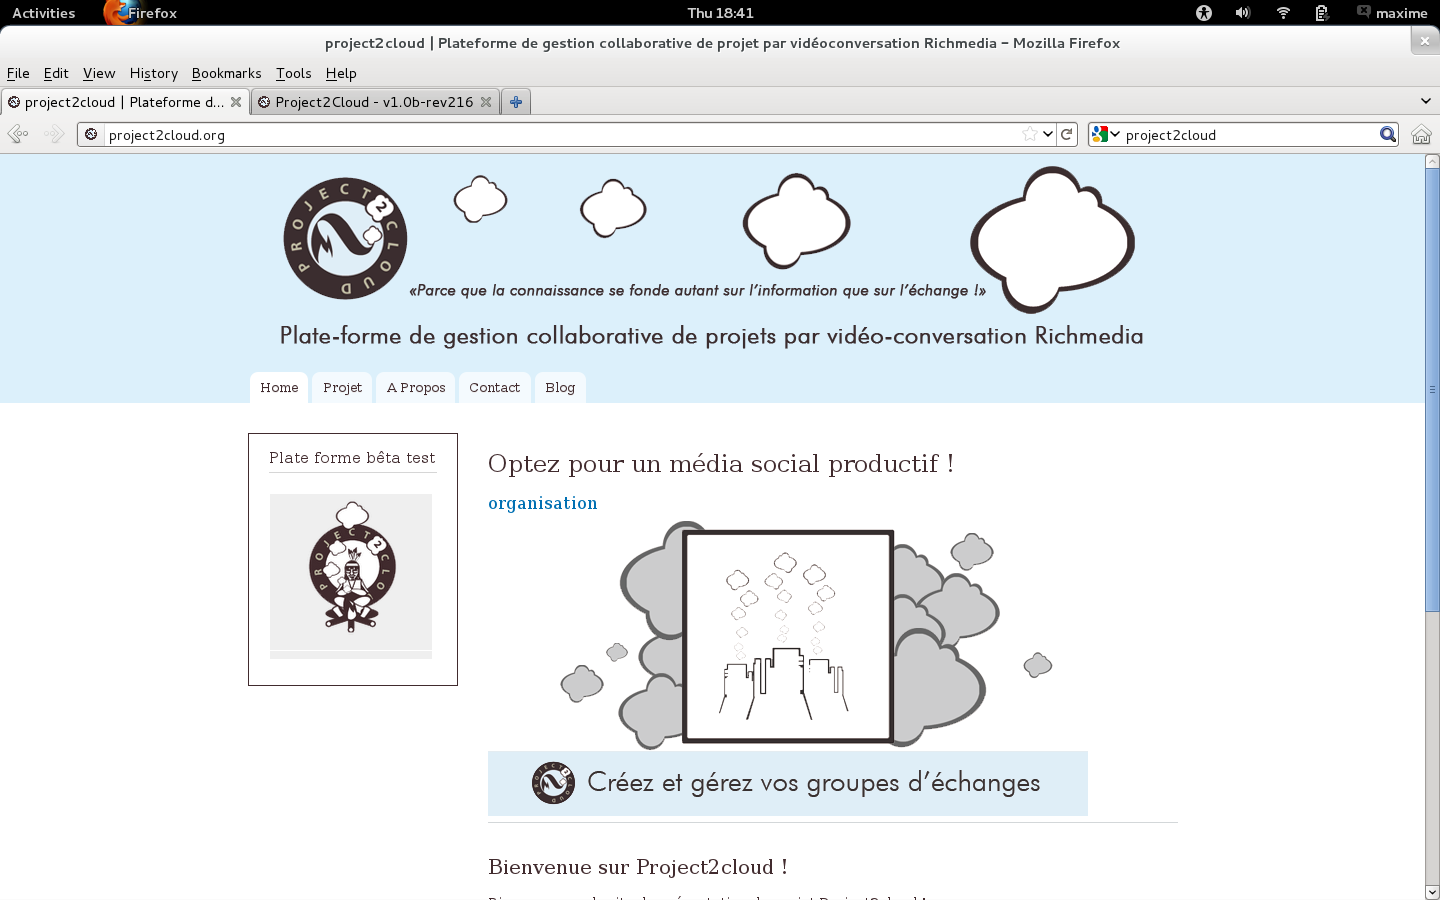
\includegraphics[width=350pt]{site}
					\caption{Site de présentation de l'application.}			
				\end{center}
			\end{figure}

			\begin{figure}[H] 
				\begin{center}
					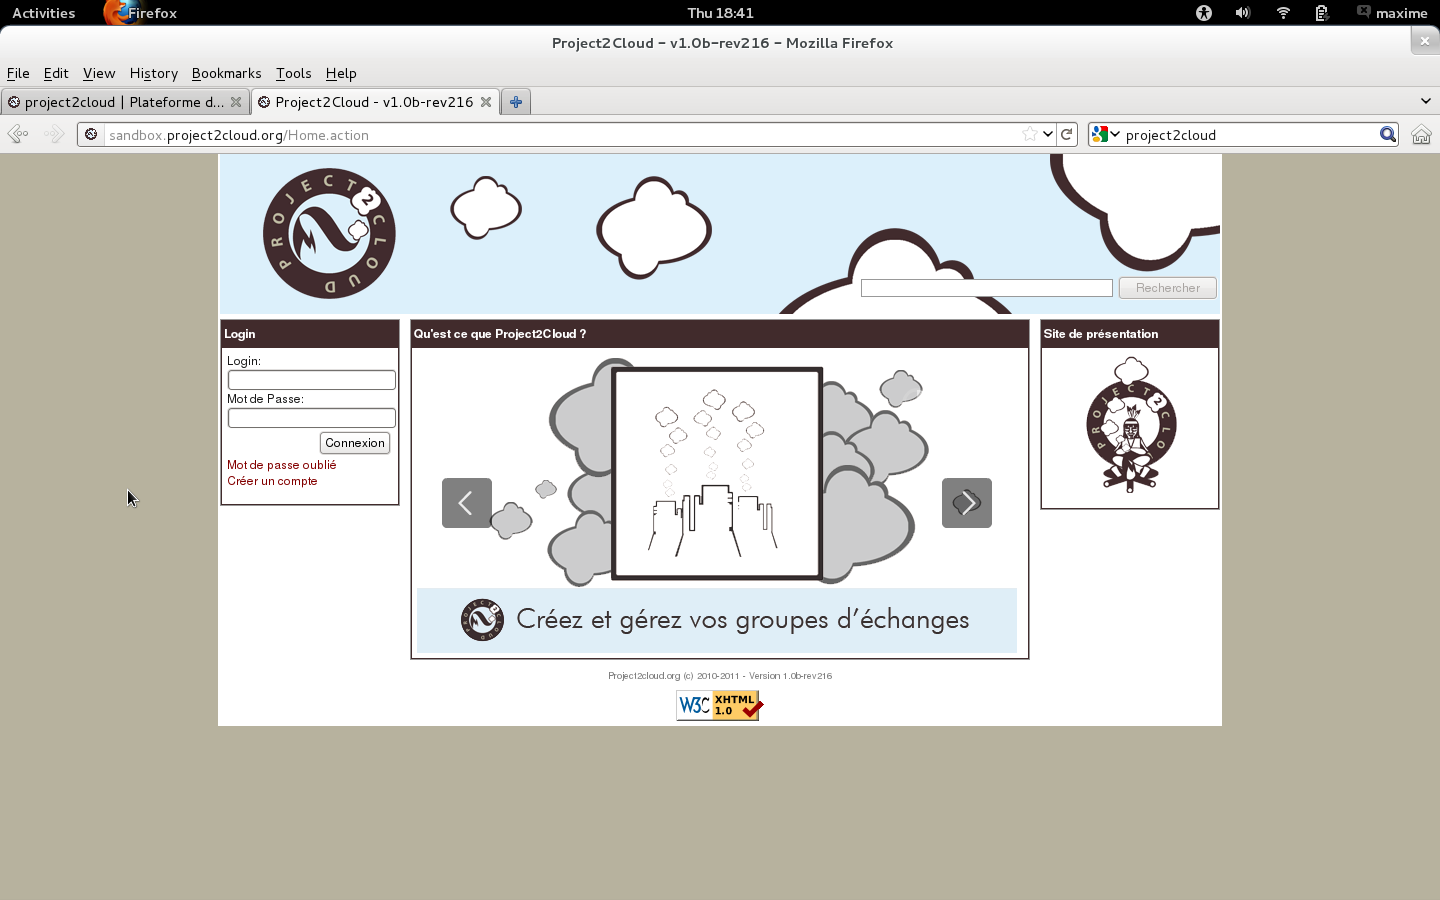
\includegraphics[width=350pt]{plateforme_d_essai}
					\caption{Plateforme Project2Cloud.}			
				\end{center}
			\end{figure}
			
\begin{figure}[H] 
				\begin{center}
					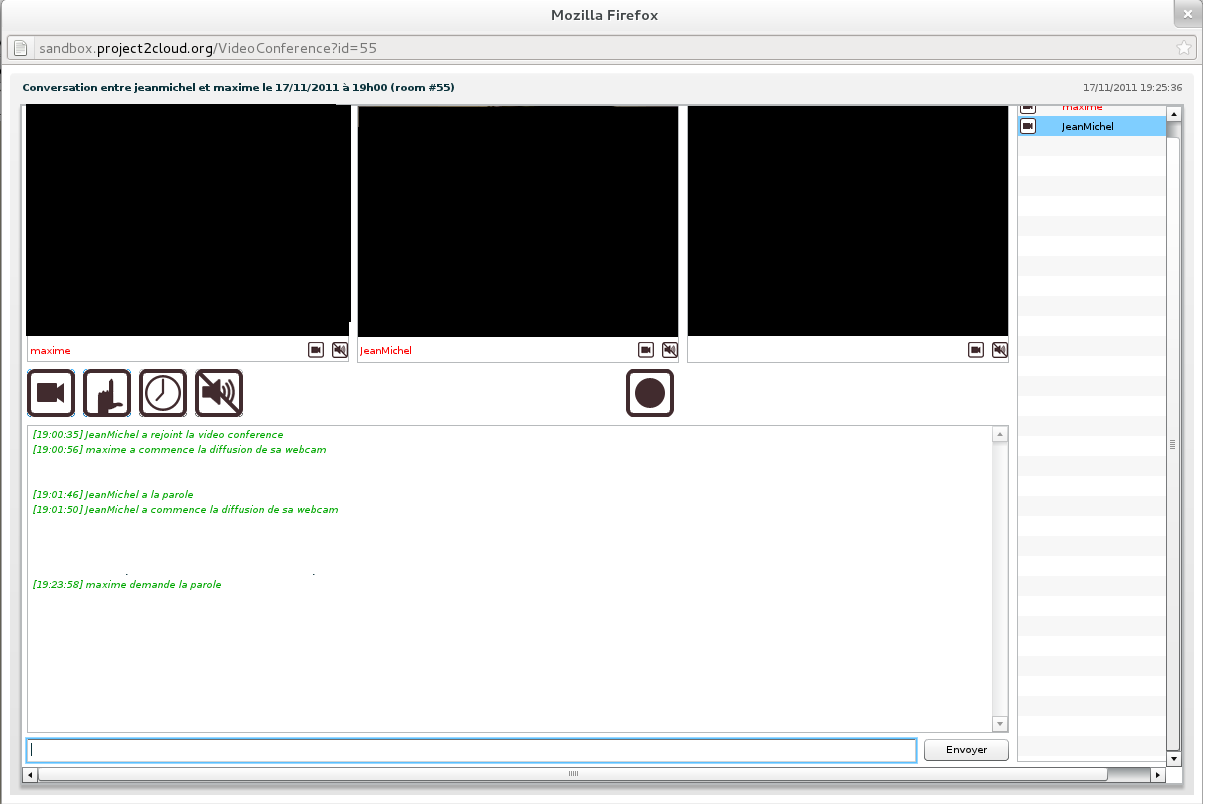
\includegraphics[width=350pt]{videoconf}
					\caption{Conférence vidéo sous Project2Cloud.}			
				\end{center}
			\end{figure}

			\subsection{Contexte du travail}
			Notre projet a pour but d'amener une nouvelle fonctionnalité parmi celles citées précédemment. Celle de retranscrire les conversations des sessions, et ainsi de faciliter l'indexation des conférences vidéos. 

			%\subsection{Division du travail en événements métier}
			
			
			\subsection{Portée du produit (cas d’utilisations)}
			Les cas d'utilisation présentés seront ceux en rapport avec notre projet. Il ne prendront pas en compte les cas d'utilisation de la plateforme déjà existante. Pour la partie transcription de texte, notre module devra recevoir le fichier son encodé par la plateforme et le convertir en fichier texte. Il devra également y associer un fichier XML dans lequel les mots clés de la conversation seront indexés grâce une timeline. Une fois le texte transcrit, ce dernier devra être pris en charge par le serveur. Le serveur devra enregistrer le texte ainsi que l'indexation pour en garder la trace. 

			\begin{figure}[H]
				\begin{center}
					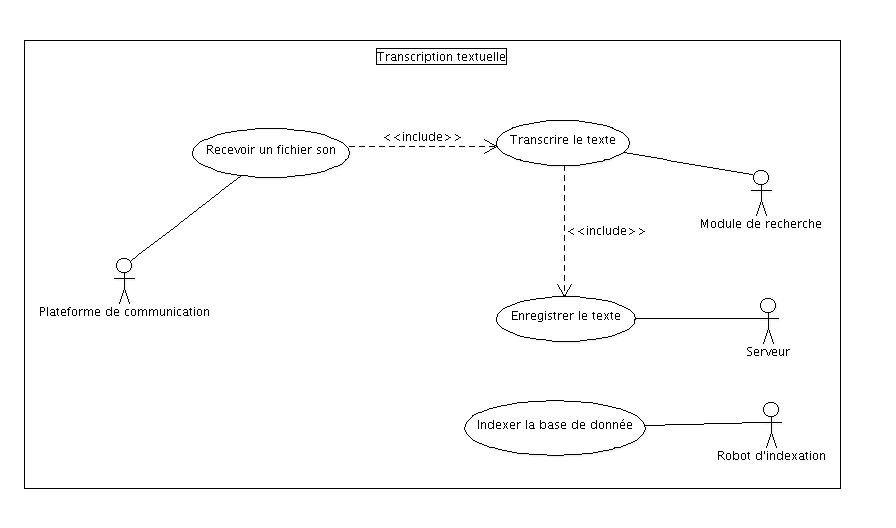
\includegraphics[width=350pt]{UseCaseDiagramTransc}
					\caption{Diagramme des cas d'utilisation de la transcription vocale.}			
				\end{center}
			\end{figure}

			\begin{figure}[H] 
				\begin{center}
					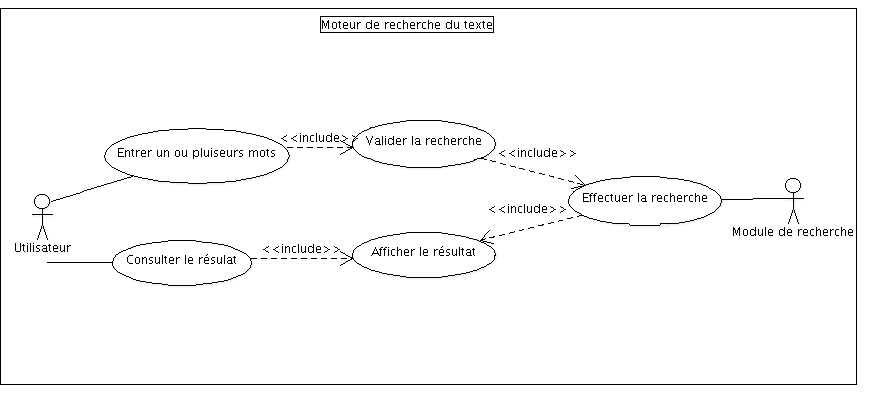
\includegraphics[width=350pt]{UseCaseDiagramMoteur}
					\caption{Diagramme des cas d'utilisation du moteur de recherche.}			
				\end{center}
			\end{figure}

			

			%\subsection{Limites du produit : diagramme de cas d’utilisation}
			

			%\subsection{Description sommaire des cas d’utilisation}
			

		\section{Exigences fonctionnelles et exigences sur les données}

			\subsection{Exigences fonctionnelles}
			Le projet sera basé sur le traitement de fichiers sonores. 
				\subsubsection*{Transcription du fichier son en texte}
				La transcription, ainsi que l'indexation, s'effectueront en tâche de fond. Lors de la réception du fichier son, le module transcrira la voix en texte, et grâce aux modifications apportée, indexera les mots clés dans un second fichier en leur associant leur mappage temporel.
					
				\subsubsection*{Amélioration du modèle de reconnaissance}
				La Plateforme Project2Cloud donnera la possibilité à l'utilisateur d'améliorer manuellement la transcription d'une vidéo. Lorsqu'une telle correction est disponible, le module de recherche peut alors améliorer son modèle de reconnaissance. Lorsque le modèle aura évolué, il sera intéressant de transcrire de nouveau les anciennes vidéos, pour obtenir une meilleure transcription.
				
					
			\subsection{Exigences sur les données}
			Toutes les données mises en jeu dans les modules devront s'adapter avec la plateforme. Elles devront respecter les normes imposées et ne présenter aucun risque de compatibilité. Les formats d'enregistrement et de traitement seront définis plus tard, notamment lors du choix des modules. 
			
		
	
	\chapter{Exigences non fonctionnelles}
			
	
		\subsection{L’interface}
		L'interface sera simple et répondra au mieux aux contraintes imposées. La partie transcription se fait automatiquement, sans intervention de l'utilisateur. Il n'y a donc pas d'interaction avec le client pour cette partie. La partie interrogation, quant à elle, doit être intuitive et facile d'accès pour n'importe quel type d'utilisateur. L'interface n'a pas encore été décidée, elle le sera plus tard, et sera fonction du temps réservé à cette partie du projet. 
	
		\subsection{Le style du produit (packaging inclus)}
		Le produit livré au client n'aura pas de "style" particulier". Les modules seront développés indépendamment de la plateforme, et y seront rattaché en fin de projet. Il n'est donc pas nécessaire d'inclure une notion de style dans notre projet.
	
	
	\section{Facilité d’utilisation et facteurs humains}
		\subsection{Facilité d’utilisation}
		La partie transcription ne sera pas visible pas l'utilisateur. Il interagira avec la plateforme Project2Cloud comme il le ferait actuellement, puisque la transcription se fera automatiquement, sans aucune intervention de sa part. La facilité d'utilisation de cette partie de notre projet est donc fonction de la facilité d'utilisation actuelle. 
		 
	
		\subsection{Personnalisation et internationalisation}
		Le module ajouté à la plateforme ne sera pas personnalisable par l'utilisateur. L'interface et les fonctionnalités mis en place sur la plateforme ne pourront pas être modifiés. 	
		La langue de base de la plateforme est le français. Le site internet est entièrement rédigé en français et ne propose pour le moment pas d'autre langue. Le projet à pour but de ne reconnaitre que des voix françaises, sans proposer d'alternative dans d'autres langues. Il n'y a donc pas de projet d'internationalisation pour le moment. 
	 
	
	
		\subsection{Exigences d’accessibilité}
		Le projet étant intégré dans une plateforme déjà existante, les exigences d'accessibilité seront les même qu'actuellement.
	
	
	\section{Fonctionnement du produit}
		\subsection{Rapidité d’exécution et temps de latence}
		La transcription n'a pas besoin d'avoir un temps d'exécution rapide puisqu'elle se fera automatiquement sur un serveur. 

		
		\subsection{Précision et exactitude}
		La transcription se devra d'être la plus précise possible. Le degrés de précision dépendra cependant de la qualité du module sélectionné.   Éventuellement, plusieurs possibilités de transcriptions pourront être sauvegardées. Le moteur d'interrogation devra prendre en compte que les transcriptions ne sont pas toujours correctes, et donc faire une recherche avec des mots phonétiquement proches.
	
		\subsection{Fiabilité et disponibilité}
		Le projet devra être entièrement fiable et répondre au mieux à la demande du client. La qualité de la transcription ne sera pas en rapport avec le bon fonctionnement du module. Aucune erreur grave ne devra survenir pendant la transcription, sous peine de perdre complètement l'intérêt du projet. La partie recherche devra elle aussi être fiable et sans aucune erreur fatale. 
	
		\subsection{Robustesse ou tolérance à un emploi erroné}
		La qualité de la transcription dépendra du module sélectionné mais également de la qualité de parole de l'utilisateur. Une locution claire et articulée est conseillée pour un résultat optimal. Dans le cas d'une locution médiocre ou d'une mauvaise qualité du son d'entrée, les résultats seront erronés et ne peuvent pas être connus à l'avance. 
		Pour la partie recherche, le module prendra en compte toutes les erreurs potentielles que pourrait commettre l'utilisateur (saisie d'un mot inexistant, validation de la recherche sans mot écrit dans la zone de recherche...). Le module interagira dans ce cas avec l'utilisateur pour lui indiquer la nature de son impair. 
 
		\subsection{Capacité de stockage et montée en charge}
		A ce stade du projet, nous ne connaissons pas encore les capacités limites de stockage et la montée en charge du projet. 
	
		\subsection{Adaptation du produit à une augmentation de volume à traiter}
		Le projet devra pouvoir gérer une augmentation de volume d'utilisateurs. Quelque soit le nombre d'utilisateurs connectés simultanément, le module devra être en mesure d'offrir la même qualité de service à tous.  
	
		\subsection{Longévité}
		Le projet devra être opérationnel sur la durée que le client jugera nécessaire. C'est à lui que reviendra le choix de la longévité du produit. Les modules développés devront aussi être adaptables dans le temps, pour une éventuelle amélioration future. La longévité du projet déprendra donc aussi de sa qualité de réutilisation (code source commenté, documentation explicite et complète...).
	
	\section{Adéquation du produit avec son environnement}
		\subsection{Environnement physique prévu}
		Le projet sera intégré directement dans une plateforme existante. Il devra donc parfaitement s'intégrer avec le site internet hôte.
	
		\subsection{Environnement technologique prévu}	
		L'environnement technologique sera uniquement le web. 
	
		\subsection{Applications « partenaires » (avec lesquelles le produit doit collaborer)}
		Le projet n'a pas pour but de collaborer avec des applications autres que la plateforme hote qui le reçoit. 
	
		\subsection{Approche « produit » prêt à être commercialisé}
	
	
	\section{Maintenance, support, portabilité, installation du produit}
		\subsection{Maintenance du produit}
		Une fois le produit livré et validé par le client, la maintenance ne sera plus assurée dans le cadre du projet transversal. 
	
		\subsection{Conditions spéciales concernant la maintenance du produit}
		Aucune condition spéciale concernant la maintenant n'est à définir dans le cadre du projet. 
	
		%\subsection{Exigences en matière de support}
	
		%\subsection{Exigences de portabilité}
	
		\subsection{Installation du système}
		A ce stade du projet, nous ne sommes pas en mesure de répondre à cette section du cahier des charges. 
	
	
	\section{Sécurité}
		\subsection{Accès au système}
		A ce stade du projet, nous ne sommes pas en mesure de répondre à cette section du cahier des charges. 	

		\subsection{Intégrité}
		A ce stade du projet, nous ne sommes pas en mesure de répondre à cette section du cahier des charges. 

		\subsection{Protection des données à caractère personnel}
		Les données à caractère personnel ne sont pas directement liée à notre projet. Ces données sont gérées par la plateforme en place. 
	
		\subsection{Audit et traçabilité}
A ce stade du projet, nous ne sommes pas en mesure de répondre à cette section du cahier des charges. 
	
		\subsection{Protection contre les infections}
		A ce stade du projet, nous ne sommes pas en mesure de répondre à cette section du cahier des charges. 
	
	
	\section{Exigences culturelles et politiques}
		\subsection{Exigences culturelles}
		Aucune exigence culturelle n'est spécifiée pour ce projet.
	
		\subsection{Exigence politiques}
		Aucune exigence politique n'est spécifiée pour ce projet.
	
	
	\section{Lois et standards influençant le produit}
		\subsection{Conformité avec la loi}
		Le projet sera conforme avec la loi et les exigences juridiques française. 
	
		\subsection{Conformité avec des standards}
		A ce stade du projet, nous ne sommes pas en mesure de répondre à cette section du cahier des charges. 

	\chapter{Autres aspects du projet}
		\section{Questions sans réponse}
		
		\section{« COTS » : Progiciels ou composants commerciaux}
		A ce stade du projet, nous ne sommes pas en mesure de répondre à cette section du cahier des charges. 

		\section{Nouveaux problèmes, créés par l’apparition du nouveau système}
		A ce stade du projet, nous ne sommes pas en mesure de répondre à cette section du cahier des charges. 

		\section{Tâches à faire pour livrer le système}
		A ce stade du projet, nous ne sommes pas en mesure de répondre à cette section du cahier des charges. 

		\section{Contrôle final de qualité sur site (Cutover)}
		A ce stade du projet, nous ne sommes pas en mesure de répondre à cette section du cahier des charges. 

		\section{Risques liés au projet}
		Les risques éventuels liés au projet seront découverts au moment de la partie de conception, et dépendront du langage informatique utilisé. 

		\section{Estimation des coûts du projet}
		Le projet n'aura aucun coût spécifique. 

		\section{Manuel utilisateur et formations}
		Les manuels utilisateurs et formations seront conçus au fur et à mesure de l'avancement du projet. 

		\section{Salle d’attente : idées pour les futures versions}
		Les idées pour des versions futures n'ont pas été abordées. Elles le seront dans le cas où l'avancement du projet le permettrait, et résulteraient d'un accord entre les tuteurs enseignants et le maître d'ouvrage.
	
	
	%------------------------------------------------- IV. BiBliographie -------------------------------------------------%
	
	%------------------------------------------------- BiBliographie -------------------------------------------------%
	
	\part{Étude bibliographique}
	\parttoc
	
	\setcounter{chapter}{0} % Pour recommencer la numérotation des chapitres à 1
	\setcounter{section}{0} % Pour recommencer la numérotation des section à 1
	
	\renewcommand*{\theHchapter}{\thepart.\thechapter}
	\chapter{Transcription automatique d'un fichier audio vers un fichier texte}
	\section{Principe de fonctionnement de la reconnaissance automatique de la parole}
	La reconnaissance de la parole (RAP) est une forme de reconnaissance de forme, et suit donc le même type de procédure~\cite{invited-paper}. Ce dernier commence par la capture d'un signal correspondant au signal entrant enregistré par un locuteur lorsque celui-ci parle dans un microphone. Ces données sont par la suite compressées. Cette étape est primordiale pour pouvoir, d'une part travailler dans des temps raisonnables et d'autre part, permettre au processus de reconnaissance de se concentrer sur les aspects pertinent du signal. En effet, il est inutile de garder toutes les données, puisque beaucoup d'entre elles sont inutiles pour la RAP. Cependant, c'est aussi une étape très sensible, car une mauvaise compression peut également amener à perdre des informations primordiales au bon fonctionnement de la RAP. Vient ensuite la recherche de caractéristique dans le signal. On cherche ainsi à trouver un modèle ce rapprochant au maximum de ces caractéristiques. Enfin, il faut prendre une décision sur le modèle qui minimise au mieux et le coût, et les erreurs. 
	
	\section{Difficultés de l'analyse de la parole}
	De nombreux obstacles s'opposent à une bonne reconnaissance automatique de la parole.
	\subsection{Décompositions de la paroles en phonèmes}
	\subsubsection{Qu'est ce qu'un phonème ?}
	La parole est une succession de sons, que l'on identifie comme étant des phonèmes. Un phonème est en fait la plus petite unité d'un mot : un mot est constitué de syllabes, qui sont elles même constituées de phonèmes. Par exemple le mot "être" est constitué d'une seule syllabe, en revanche, il est constitué de trois voir quatre phonème (dépendant du fait que le locuteur prononce le 'e' final ou pas). Ces phonèmes sont représentés entre slash, de la même manière que les symboles de phonétique. Dans notre exemple nous avons donc les phonèmes suivant : \textipa{/E/}, \textipa{/t/}, \textipa{/r/} et éventuellement \textipa{/e/} .
	
	Le contenu basique de la parole est donc une séquence de phonèmes, qui une fois décodés, sont traduit par une séquence de mot grâce à une correspondance dans un dictionnaire.
	\subsubsection{Caractéristiques des phonèmes}
	Les phonèmes sont caractérisé par trois paramètres :
	\begin{itemize}
		\item{le mode d'articulation}
		\item{la place de l'articulation}
		\item{la voix}
	\end{itemize}
	Cependant par la suite, nous ne nous intéresserons dans le cadre de la RAP qu'au mode d'articulation.
	
	Le mode d'articulation correspond au type de son, que nous pouvons classer en 5 groupes majeurs :
	\begin{itemize}
		\item{Consonne occlusive : elle fait intervenir un blocage complet de l'air, suivit d'un relâchement soudain (i.e. /p,t,k,b,d,g/)}
		\item{Consonne fricative : l'air passe par une fente, formée par le rapprochement des lèvres, des dents, et/ou de la langue avec les lèvres/dents (i.e. /f,s,v,z/)}
		\item{Consonne nasale : il y a blocage complet, mais à l'inverse d'une consonne occlusive, l'air passe par le nez (i.e. /m,n/)}
		\item{Voyelles : pas d'obstruction de l'air, seule l'emplacement et la forme de la langue et des lèvres modifient le son}
		\item{Consonne latérale (ou liquide) et semi-voyelle : le premier correspond aux consonnes pour lesquelles l'air s'échappe par les côtés de la langue, et le second, aux lettres qui donne un son voyelle, mais sont pourtant caractérisées comme étant des consonnes(i.e. /l,r,w,j/)}
	\end{itemize}
	Il est ici important de rappeler que nous nous intéressons au type de son formé, et non à une lettre. Par exemple, ici la lettre 'c' n'est pas référencée, puisqu'elle se rapporte à deux sons : le son /k/ (e.g. dans le mot "caractère") et le son /s/ (e.g. dans le mot "ceci"). De la même manière, pour le groupe des sons voyelles, il ne faut pas se restreindre aux six voyelles de la langue française, puisque bien d'autres sons de type voyelle existent (e.g. \textipa{/\oe/} dans "oeuf", \textipa{/E/} dans "lait").
	
	Les systèmes de RAP n'ont pas de grandes difficultés à classer ces groupes de phonèmes, tout du moins lorsqu'il s'agit des groupes de consonnes occlusives, fricatives et de voyelles. En effet, ces sons ont de fortes caractéristiques, notamment une forte énergie périodique. Or ceci est une information primordiale car la détection de périodes est un facteur majeur de la RAP.
	
	
	
	\subsubsection{La coarticulation}
	Un phonème isolé est assez facile à identifier pour un système de RAP. Seulement, lorsque nous parlons, nous ne saccadons pas nos paroles en son. Nous enchainons les phonème, les mots, les uns après les autres, d'une manière plus ou moins fluide. C'est dans ce contexte qu'apparaît le principe de coarticulation.
	
	Un phonème intervient de façon significative sur le phonème qui le suit, mais également sur le phonème qui le précède. En effet, l'appareil vocal humain est fait de telle manière qu'il est impossible de passer d'un phonème à un autre (i.e. d'un son à un autre) instantanément. Pour chaque enchainement de phonèmes, il y a un moment de transition (plus ou moins importante et plus ou moins détectable). Pendant celle-ci, la forme des lèvres et la position de la langue et de la mâchoire vont se modifier, pour correspondre au prochain phonème. Par exemple, pour passer d'un son /s/ à un son /t/, la transition est le moment où l'on commence à avancer la langue jusqu'à ce que celle-ci touche les dents. Bien que difficilement détectable pour l'oreille humaine, cette transition apparait très clairement en terme de signal.
	
	De plus, dans la langue française, les règles de grammaires veulent que nous fassions les liaisons entres les mots, faisant ainsi apparaître des phonèmes.
	
	Ces deux phénomènes de coarticulation et de liaisons rendent la RAP très complexe, puisque un dictionnaire va associer à un mot les phonèmes qui le composent, et non les transitions. Ces transitions ne sont pas identifiables en terme de phonème et sont différentes pour chaque personne (vitesse de parole, appareil vocale différent, etc...). Il faut donc que le système de RAP apprennent à ne pas prendre en compte ces transitions. La liaison quant à elle est un tout autre problème, car elle fait apparaître des phonèmes tout à fait identifiable, "modifiant" ainsi les mots. C'est donc une nouvelle contrainte qui s'ajoute pour la RAP. Il est en effet parfois difficile de distinguer ces liaisons comme étant réellement des liaisons, e.g. "on en" et "on n'en". Nous pouvons en déduire qu'une reconnaissance simple des phonèmes n'est pas suffisante pour une bonne RAP : il faut y associer toutes les règles de grammaire de la langue.
	
	
	\subsection{Variabilité de la parole}
	Beaucoup de variabilité dans l'aspects de la parole peuvent intervenir et ainsi perturber la RAP~\cite{speech-variability}
	\begin{itemize}
		\item la physiologie de chaque individu : chacun individu est unique, et il en va de même pour son appareil vocal. En conséquence, chaque son produit par un individu est unique. Il faut donc un système de RAP suffisamment performant pour réussir à trouver une ressemblance dans un même phonème prononcé par différente personne.
		\item Les accents étrangers et régionaux : la langue d'origine influe inévitablement sur la prononciation, ainsi un espagnol par exemple aura tendance à rouler ses 'r' en français, ce qui change le phonème, créant une séquence de phonème qui ne peut pas être associé à un mot. De la même manière, pour les accents régionaux, bien que la langue reconnue est leur langue d'origine, ces individus ont un accent qui vient également changer certains phonèmes, et qui vient même en rajouter (e.g. l'accent marseillais). Pour ce cas, il faut un système qui soit capable de repérer que tel ou tel individu à tendance à prononcer ces phonèmes de telle manière.
		\item La vitesse de parole : tout le monde parle à sa vitesse, et cela complique d'avantage une bonne RAP, puisqu'entre deux individus, un qui parle lentement, et le second qui parle vite, la longueur des phonèmes varie énormément.
		\item L'état émotionnel : nous sommes humains, nous avons donc toute une panoplie d'émotions qui peuvent faire varier notre parole. Une personne en colère a tendance à parler fort et vite, supprimant ainsi certains phonèmes. Une personne sous pressions, stressée, a la gorge serrée, ce qui modifie les phonèmes.
		\item etc.
	\end{itemize}
	
	On voit donc ici que beaucoup d'élément peuvent venir perturber la RAP, même pour une unique personne. Suivant les instants, cette personne peut parler plus ou moins vite, se mettre en colère, etc... Si l'on y rajoute une personne avec un accent, qui est elle même sujette à toutes ces variations, on se rend compte de l'extreme complexité pour établir un bon système de RAP.
	
	
	
	\section{Variantes du problème de la reconnaissance de la parole}
	
	\subsection{Locuteurs connu et inconnu}
	Il existe deux types majeurs de systèmes de RAP :
	\begin{itemize}
		\item Locuteur connu
		\item Locuteur inconnu
	\end{itemize}
	
	\subsubsection{Locuteur connu}
	Ce type de système est le plus répandu, car il est le plus facile à réaliser. Il requiert une période d'entrainement (i.e. de réglage) pendant laquelle il lit des phrase à voix haute des phrases que lui indique le logiciel. Ainsi, ce dernier apprend la manière de parler de l'utilisateur. Il possède une base de données de phrase (qui sont choisies pour leur diversité de phonèmes), et sachant ce que l'utilisateur va dire, il peut associer chaque son à sa signification.
	
	\subsubsection{Locuteur inconnu}
	Ce deuxième type de système, quant à lui, est immédiatement opérationnel. Il ne requiert aucune période d'entrainement, et apprend seul, au fur et à mesure que l'utilisateur parle, à identifier ses phonèmes.
	
	\subsubsection{Analyse}
	Lorsque l'utilisateur est connu, le système donne souvent de bien meilleur résultat. Cependant, il présente un inconvénient majeur : une importante perte de temps pour l'utilisateur. De plus, son principe même a de fortes lacunes. En effet, ce type de système fait \textbf{lire} l'utilisateur alors que pendant son utilisation, les chances sont grandes que le locuteur parle spontanément plutôt que ne lise. Cependant, il est montré qu'en terme de signal, les phrases lues et les phrases parlées spontanément sont complètement différentes~\cite{read-spontaneous}.  La spontanéité demande plus de réflexion, et il plus d'émotion lorsque nous parlons que lorsque nous lisons. De plus, lorsque nous parlons spontanément, l'espace spectral se réduit, et plus la parole est spontanée, plus la réduction est importante (comme le montre la figure \ref{reduction_rate_phoneme_read_spontaneous}). Or une réduction de l'espace spectral provoque une réduction de la précision de reconnaissance de phonème, ce qui implique une réduction de la RAP.
	
	\begin{figure}[H]
		\begin{center}
			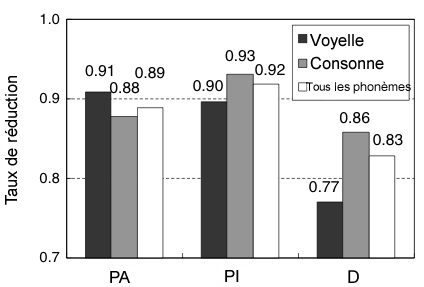
\includegraphics[width=10cm]{reduction_rate_phoneme_read_spontaneous}
			\caption{Moyenne du taux de réduction des voyelles, consonnes et tous les phonèmes pour les types PA, PI et D de paroles, respectivement Présentation Académique, Présentation Improvisée et Discours, par rapport à des phrases lues. \cite{read-spontaneous}}
			\label{reduction_rate_phoneme_read_spontaneous}
		\end{center}
	\end{figure}
	
	\subsection{Vocabulaire connu et limité ou vocabulaire large}
	Pour certains systèmes, le besoin de vocabulaire est très limité, et le système en perd en complexité. Par exemple, les répondeurs à reconnaissance automatique de la parole ne demandent que très peu de mots : "oui", "non", "suivant", "supprimer"... Il sont donc beaucoup plus facile à coder, puisque la suite de phonème ne correspond qu'à un mot, et les possibilités sont très rapides à parcourir.
	
	En l'occurrence, notre projet requiert un vocabulaire très large, puisqu'il doit pouvoir identifier tous les mots qui peuvent survenir lors d'une conversation entre différentes personnes. Cependant, même avec un vocabulaire extrêmement complet, il arrive couramment que des mots inconnus soient prononcés (e.g. nom propres, jargon scientifique, etc.)~\cite{retrieval-browsing-spoken-content}, et si un mot n'est pas dans le dictionnaire, alors la transcription sera forcément fausse. Pour palier à ce problème, plusieurs solutions existent. La première consiste à proposer à l'utilisateur plusieurs hypothèses, avec la possibilité d'ajouter un mot (i.e. de la même façon qu'il est possible d'ajouter des mots aux correcteurs orthographiques de logiciels de bureautique). Néanmoins, cette solution n'est pas envisageable pour notre projet, car ces vidéos seront faites lors de réunions professionnelles, et il n'est donc pas possible d'interrompre l'utilisateur pour chaque mot que le logiciel n'arrive pas à identifier. La deuxième solution, quant à elle, propose de rechercher les mots inconnus dans les documents associés à la vidéo. Cette dernière semble tout à fait appropriée à notre projet, puisqu'il est prévu que pour chaque réunion (i.e. visio-conférence) lui soit associé en plus de la vidéo et de l'audio, les documents utilisés lors de cette dernière. Il serait donc possible de parcourir ces documents afin d'éventuellement trouver le mot correspondant. Cependant, cette proposition ne peut pas fonctionner systématiquement, puisque d'une part, il n'est pas obligatoire que des documents aient été utilisés lors de la réunion, et d'autre part, quand bien même des documents auraient été partagés, les mots inconnus ne sont pas forcément contenu dans ces documents. Pour ce problème, nous pouvons proposer une troisième solution, qui consiste à faire une première passe du contenu parlé avec un tout autre système pour essayer d'en retirer le sujet de la vidéo, et ainsi créer un vocabulaire spécifique à ce sujet. Cette solution pourrait éventuellement faire l'objet d'une amélioration future par l'entreprise, mais elle ne sera pas employée pour notre projet.
	
	
	\subsection{Découpage temporel en locuteurs}
	Lorsque plusieurs locuteurs sont présents, il est intéressant de découper le flux de paroles en locuteurs. En effet, un bon modèle s'adapte au locuteur, or si nous ne différencions pas les différents locuteurs, le style de parole changeant à chaque prise de parole, il sera impossible au système de s'adapter convenablement. Ainsi, en découpant en locuteur, le système peut avoir plusieurs "adaptation" pour correspondre à chacun des locuteurs.
	
	Il n'est pas prévu de mettre cette fonctionnalité dans le projet pour l'instant, puisque nous partons du point de vue qu'il n'y a qu'un seul individu de chaque côté des micros. Dans ce contexte, la division est très simple, puisqu'une entrée correspond à un locuteur. Cependant, à terme, il doit être possible d'avoir plus d'une personne pour un micro, il y a donc une chance que l'entreprise nous demande d'inclure cette fonctionnalité.
	
	\subsection{Qualité acoustique de la composante parole}
	La précision de la RAP peut très vite chuter si la qualité audio est mauvaise, notamment s'il y a des bruits de fond~\cite{noisy-speech-recognition}, de la musique, une mauvaise transmission, etc.
	
	
	
	
	\chapter{Recherche d'information dans des documents parlés}
	\section{Son intérêt}
	L'augmentation constante de l'activité informatique et la réduction des coûts de stockage conduisent à un très fort nombre de données de tout types, échangées et stockées. En conséquence, la recherche de données est devenue un domaine clé, tout particulièrement celui de la recherche de données textuelles, qui est le plus courant~\cite{retrieval-browsing-spoken-content}.
	
	La recherche de document parlé, quant à elle, ne s'est pas beaucoup développée au fil des années, notamment dû à son manque de demande et d'exactitude. Cependant, dans les dernières année, l'explosion de contenu audio/vidéo disponible sur internet en fait un important outil. Néanmoins, ce domaine a nécessite encore beaucoup de progrès, car les résultats ne sont pas à la hauteur des exigences des utilisateurs. En effet, l'idéal serait de faire la recherche dans une transcription alignée avec l'audio, ce qui simplifierait le problème en une recherche textuelle. Malheureusement, dans cette hypothèse, le texte devrait être une transcription exacte de l'audio, ce qui nécessiterait une transcription manuelle. Or cette dernière prend du temps, et donc coûte cher. C'est dans ce contexte qu'intervient la recherche d'information des documents parlés.
	
	\section{Sa difficulté}
	Lorsque l'on crée un système de RAP pour une recherche d'information, le choix du dictionnaire est primordial. En effet, en général, le vocabulaire d'un ASR est assez restreint. Or, si un mot est prononcé et n'est pas dans le dictionnaire, alors le système de RAP de le reconnaitra jamais correctement, et les requêtes d'utilisateur contenant ce(s) mot(s) échoueront systématiquement. Malheureusement, les mots ou groupes de mots recherchés sont souvent les moins courants et les plus spécifiques à un sujet, qui ne sont généralement pas présent dans les dictionnaires des systèmes de RAP.
	
	On en déduit l'importance d'un système de recherche flexible, qui accepte des solutions avec des mots plus ou moins proches.
	
	\section{Différentes méthodes}
	La méthode la plus classique est évidemment une recherche textuelle classique dans les transcriptions des vidéos. Cependant, une autre méthode suggère d'attaquer le problème sous un autre angle, en ignorant totalement le texte, et de ne s'intéresser qu'à la prononciation. Le système de RAP, à la place de produire un texte de mots, produirait un texte de prononciation phonétique. La requête de l'utilisateur serait ensuite traduite en langage phonétique, et recherchée dans les transcriptions. Le très grand avantage de cette méthode est que solutionne le problème de vocabulaire inconnu. De plus, le système de RAP serait nettement plus performant puisqu'il n'aurait qu'à traduire ce qu'il "entend" en phonétique, et non plus à rechercher de correspondance dans son dictionnaire. En revanche, la recherche de mots clés, quant à elle, serait beaucoup plus longue. Or dans notre cas actuelle, la performance du système de RAP n'a pas de réelle importance puisqu'elle se fait en tache de fond, contrairement à la recherche qui se fait en temps réel.
	
	Une seconde solution utilise les deux méthodes précédentes, combinant à la fois la recherche par mot et la recherche phonétique. L'idée serait de faire une première recherche large (i.e très flexible quant à l'exactitude de la correspondance des mots) en utilisant les mots de l'utilisateur. Viendrait ensuite une seconde passe sur ces résultats, en utilisant la phonétique. Cette méthode impliquerait donc que le système de RAP produise deux transcriptions : une textuelle et une phonétique. Cela ne pose pas de réelle contrainte, puisque comme dit précédemment, la rapidité du système RAP n'a pas d'importance. La recherche, elle, serait plus rapide qu'avec la méthode n'utilisant que la phonétique, puisqu'ici elle ne se fait que sur un nombre de documents préalablement restreint.
	
	
	
	
	
	

	
	
	
	
	
	
	
	
	
	
	
		
	\nocite{introduction-hmm}
	\nocite{tutorial-hmm}
	
	
	
	%------------------------------------------------- V. Procédure de recette -------------------------------------------------%
	
		%------------------------------------------------- Procédure de recette -------------------------------------------------%

	\part{Procédure de recette}
	
	\setcounter{chapter}{1} % Pour recommencer la numérotation des chapitres à 1
	\setcounter{section}{0} % Pour recommencer la numérotation des section à 1
	
	\section{Introduction}
	Notre projet s'intégrera dans une plateforme déjà existante. Pour le tester, nous devrons vérifier qu'il répond aux attentes fonctionnelles, mais qu'il s'intègre également correctement dans la plateforme hôte. 
	Dans ce cahier de recette nous présenterons un batterie de tests visant à faire valider par le client l'intégralité des modules présentés dans le cahier des charges. Nous présenterons ici les tests sous la forme :
	\\
	\begin{center}
		Test effectué: \textit{Résultat(s) attendu(s)}
	\end{center}
		
	
	\section{Tests d'intégration du module dans la plateforme}


	Démarrage d'une vidéo conférence sur le site "Project2Cloud" : \textit{La vidéo conférence doit démarrer sans message d'erreur ni bug.}

	Lire un texte contenant les mots clés : "test", "réunion", "projet", "conférence" : \textit{La vidéo conférence se poursuit sans interruption ni ralentissement.}


	Couper la vidéo conférence : \textit{La vidéo conférence se termine sans erreur.}


	Ouvrir le module de recherche de texte : \textit{Une interface permettant de saisir du texte doit apparaitre}


	Saisir le mot "réunion" dans la zone de texte: \textit{La zone de texte doit se remplir du mot saisi}


	Valider la recherche en cliquant sur le bouton "Rechercher" : \textit{Une nouvelle fenêtre s'ouvre et affiche l'intégralité des occurrences du mot "réunion" trouvés.}
	
	
	
	
	%------------------------------------------ VI. Estimation des charges et planifications -------------------------------------%

	%------------------------------------------ Estimation des charges et planifications -------------------------------------%

\part{Estimation des charges et planifications}
	
	
	%----------------------------------------------------- VII. Modélisation -----------------------------------------------------%

	%------------------------------------------------- Modélisation -------------------------------------------------%
	
	\part{Modélisation}
	
	\setcounter{chapter}{0} % Pour recommencer la numérotation des chapitres à 1
	\setcounter{section}{0} % Pour recommencer la numérotation des section à 1
	
	\renewcommand*{\theHchapter}{\thepart.\thechapter}
	\chapter{Introduction}
	La phase de conception est la phase permettant de mettre en place les différentes étapes nécessaires à la réalisation de notre projet. Elle inclue des schémas et des diagrammes structurés représentant les étapes et les fonctionnalités de notre future application. La phase de conception est la dernière étape avant la programmation logicielle, elle doit donc être précise et fiable, dans le but de minimiser au maximum les risques d'erreurs d'implémentation. 
	
	La phase de conception s'appuie en grande partie sur ce qui a été mis en place dans le cahier des charges de la phase 1. Les différentes réunions avec les différents protagonistes du projet ont permis de fixer les objectifs prioritaires à concevoir en priorité. Dans notre projet, il s'agira donc de trouver un moyen efficace de transcrire la voix en texte, et de pouvoir exploiter cette transcription. Pour  cela, il sera nécessaire d'établir des connexions entre notre module et le serveur de la plate-forme Project2Cloud. Nous nous sommes pour cela initié au techniques de transcription vocale ( Speech-to-text ) au travers de modules libres existant.

	 Dans ce compte rendu de phase de conception, nous présenterons le module développé sous différents aspects (diagrammes, partons de conception). Nous estimerons également la charge de travail prévue, via la méthode COCOMO. Cet méthode nous donnera des indications sur le volume de travail à fournir en fonction des choix techniques effectués avec les tuteurs enseignants et entreprise. 


	\chapter{Principe général}
	Notre module sera développé à part, et ne sera pas directement intégré dans la plate-forme P2C. Il devra cependant échanger des informations contenu sur le serveur de la plate-forme. Les vidéos enregistrées sur le serveur devront être traité par notre module, qui en proposera une transcription de type Speech-to-text. La transcription ainsi effectuée sera renvoyée au serveur. Idéalement, un système d'échange module-serveur pourrait être mis en place, permettant un dialogue continu entre les deux instances. Ceci permettrait de rendre le module auto-didacte et d'améliorer significativement la qualité de la transcription proposée. 

		IMAGE DU PRINCIPE GENERALE

	
	
	
	\chapter{Transcription}
	Le module va périodiquement interroger la base de donnée pour détecter les nouveaux fichiers son encodés disponibles. Lorsque tel est le cas, il lancera ce fichier pour le transcrire grâce à son modèle de reconnaissance. De plus, à chaque mot clé reconnu (mot clé entré pas l'utilisateur), il l'indexera dans un fichier XML. Dans ce dernier, seront associés un mot clés et une donnée temporelle, correspondant au moment où ce mot clé a été prononcé dans la vidéo.

	A chaque fichier de transcription sera associé un numéro de version. Ainsi, lorsque le modèle de reconnaissance a suffisamment évolué, une nouvelle transcription sera faite.

	Diagramme de classe de la transcription et du dialogue avec le serveur


	
	\chapter{Amélioration de modèle}
	
	
	\chapter{test}
	Notre application est composée de deux tests  :  transcription et mappage temporelle de la transcription

	\section{tests unitaires}

	\subsection{tests boite noire}
	
	
	
	
	
	

	
	
	%----------------------------------------------------- VIII. Réalisation -----------------------------------------------------%

	%------------------------------------------------- Réalisation -------------------------------------------------%
	
	\part{Réalisation}
	
	\setcounter{chapter}{0} % Pour recommencer la numérotation des chapitres à 1
	\setcounter{section}{0} % Pour recommencer la numérotation des section à 1
	
	\renewcommand*{\theHchapter}{\thepart.\thechapter}

Le rapport de réalisation est un rapport court mais qui comporte généralement des annexes longues.

Un premier chapitre décrit les outils utilisés pour la réalisation (IDE, serveur de version, logiciel de test, etc).

Un second chapitre montre le résultat du déroulement du logiciel généralement grâce à des snapshots ce qui doit prouver au lecteur ce qui fonctionne et ce qui ne fonctionne pas.

Un troisième chapitre explicite les spécificités qui ont été mises en oeuvre afin de répondre à la modélisation ou justement les écarts avec cette modélisation. Ce chapitre renvoie sur une annexe avec le code

Un quatrième chapitre explicite les tests prévus et donne un aperçu global de leurs résultats. Ce chapitre renvoie sur le document des tests détaillés (cf. chapitre suivant).

Une conclusion donne le résumé du projet et les perspectives à en tirer.

		\chapter{Outils utilisés}
		
		\section{IDE}
		Pour ce projet, nous avons utilisés trois langages de programmations différents :
		\begin{itemize}
			\item Java
			\item XML
			\item C
		\end{itemize}
		Différents IDE ont donc été utilisés.
		
		\subsection{Java}
		Pour le langage Java, nous avons utilisé la plateforme d'Eclipse. Celle-ci offre un large panel d'outils facilitant la programmation et la gestion d'erreur, rendant cet IDE un choix de prédilection.
		
		\subsection{XML}
		Le langage XML tel que nous l'avons utilisé n'étant pas très complexe, nous nous sommes contentés d'utiliser un simple éditeur de texte.
	
		\subsection{C} 
		Seul un programme a été codé en C. Nous avons utilisé l'IDE Xcode de Mac OS X pour ce programme, qui offre, de la même manière qu'Eclipse pour Java, de bon outils pour la programmation et une bonne gestion des erreurs.
		
		
		
		\section{Serveur de version}
		
		Un ser

		\chapter{Déroulement du projet}

		\chapter{Spécificités mises en oeuvres}

		\chapter{Tests prévus}

		\chapter{Conclusion}
	
	
	%----------------------------------------------------- IX. Tests -----------------------------------------------------%

	%------------------------------------------------- Tests -------------------------------------------------%
	
	\part{Tests}
	
	\setcounter{chapter}{0} % Pour recommencer la numérotation des chapitres à 1
	\setcounter{section}{0} % Pour recommencer la numérotation des section à 1
	
	\renewcommand*{\theHchapter}{\thepart.\thechapter}
	\chapter{a}
	
	Ce dossier de tests doit rendre compte de la vérification du logiciel (test unitaire, test d'intégration, recette interne)

Test unitaire :

Test d'intégration : 

Recette interne : Avant de livrer le travail au client, vous devrez effectuer vous-même la procédure de recette "en interne". Pour chaque test décrit, vous noterez le résultat obtenu, ainsi que sa conformité par rapport au résultat attendu. Lorsqu'une différence est constatée, vous la commenterez (erreur inattendue, erreur connue mais pas prioritaire, coût présumé de la mise en conformité...).
	
	
	%----------------------------------------------------- X. Manuel d'utilisation -----------------------------------------------------%

	%------------------------------------------------- Manuel d'utilisation -------------------------------------------------%
	
	\part{Manuel d'utilisation}
	
	\setcounter{chapter}{0} % Pour recommencer la numérotation des chapitres à 1
	\setcounter{section}{0} % Pour recommencer la numérotation des section à 1
	
	\renewcommand*{\theHchapter}{\thepart.\thechapter}
	\chapter{a}
	
	
	%----------------------------------------------------- XI. Dossier de dépoiement -----------------------------------------------------%

	%------------------------------------------------- Dossier de déploiement -------------------------------------------------%
	
	\part{Dossier de déploiement}
	
	\setcounter{chapter}{0} % Pour recommencer la numérotation des chapitres à 1
	\setcounter{section}{0} % Pour recommencer la numérotation des section à 1
	
	\renewcommand*{\theHchapter}{\thepart.\thechapter}
	\chapter{a}
	
	Ce dossier de déploiement de l'application doit préciser les modalités de mise en production du logiciel (installation et configuration) 
	
	
	%----------------------------------------------------- XII. PV de recette -----------------------------------------------------%

	%------------------------------------------------- PV de recette -------------------------------------------------%
	
	\part{PV de recette}
	
	\setcounter{chapter}{0} % Pour recommencer la numérotation des chapitres à 1
	\setcounter{section}{0} % Pour recommencer la numérotation des section à 1
	
	\renewcommand*{\theHchapter}{\thepart.\thechapter}
	\chapter{a}
	
	
	%----------------------------------------------------- XIII. Dimension commerciale -----------------------------------------------------%

	%	%--------------------------------------------------- Dimension commerciale ------------------------------------------------%

	\part{Dimension commerciale}
	
	\setcounter{chapter}{1} % Pour recommencer la numérotation des chapitres à 1
	\setcounter{section}{0} % Pour recommencer la numérotation des section à 1
	
	\section{Introduction}
	Le projet transversal est issu de la collaboration de l'école polytechnique de l'université de Nantes et de l'entreprise Project2Cloud. Il sera mené de bout en bout par deux étudiants de quatrième année du cycle ingénieur, supervisés par deux professeurs référents. Il s'étendra de septembre à mai. L'objectif est de permettre aux étudiants en charge de réaliser un projet professionnel dans le cadre de leurs études. Au delà de la dimension technique, les projets informatiques intègres des notions plus larges et plus actuelles. Il est donc important de prendre conscience que les projets transversaux présentent des enjeux marketing et écologiques. Il conviendra donc de mettre en œuvre une démarche organisationnelle, qui s'appuiera sur les enseignements dispensés dans les modules Homme Entreprise Société. 
	Nous commencerons par présenter l'entreprise, puis nous détaillerons le projet qui nous a été proposé. Nous terminerons par la problématique marketing que nous avons décidé de développer. 

	\section{L'entreprise : Project2Cloud}
	Project2Cloud est une plate-forme de gestion collaborative. Une site de présentation est déjà en ligne à l'adresse http://project2cloud.org/. Elle propose différents services de communication, tels que la vidéo-conférence, le chat et la conversation audio. Le but est d'offrir aux utilisateurs un panel complet de communication, leur permettant d'échanger en temps réel des informations et des services. Project2Cloud innove également avec la possibilité d'associer aux sessions de dialogue des documents de différents types (texte, vidéos...). Le document associé à la session permet de créer une "mémoire" numérique du document, autour de laquelle de nouvelles connaissances peuvent venir s'ajouter à tout moment. 

			\begin{figure}[H] 
				\begin{center}
					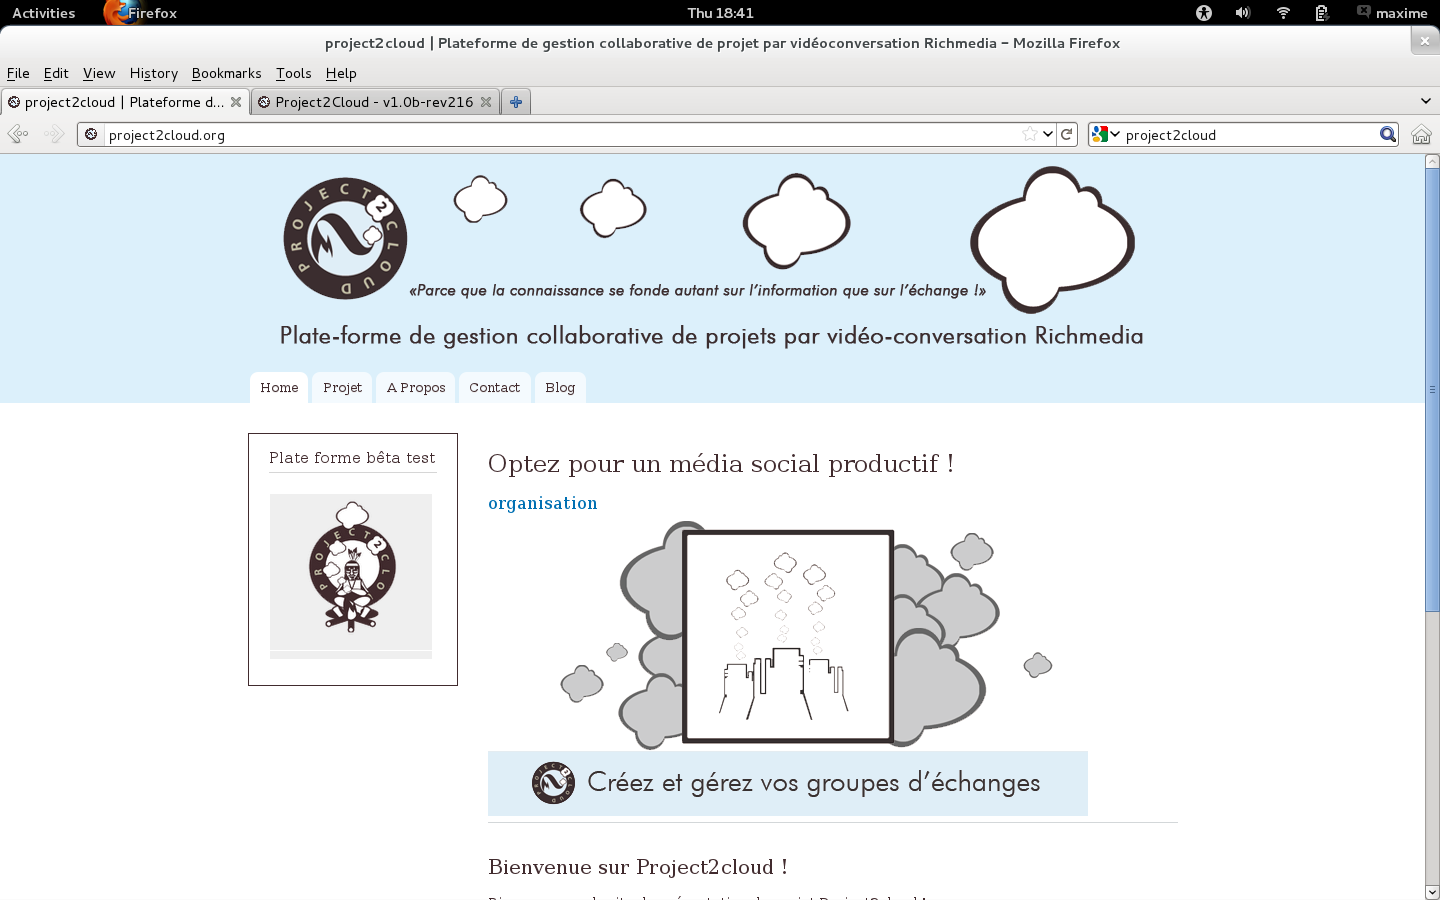
\includegraphics[width=350pt]{site.png}
					\caption{Site de présentation de l'application.}			
				\end{center}
			\end{figure}

	P2C (abréviation courante de Project2Cloud) est géré par trois informaticiens passionnés depuis maintenant 1 an. La plate-forme P2C est pour le moment en béta-test privé, c'est à dire qu'elle n'est pas encore accessible. Elle est actuellement testée par plusieurs industriels. Pour les besoins du projet, un accès nous a été donné à la version opérationnelle de la plate-forme. Cette version nous permet d'avoir une idée de l'application qui sera prochainement disponible. 

			\begin{figure}[H] 
				\begin{center}
					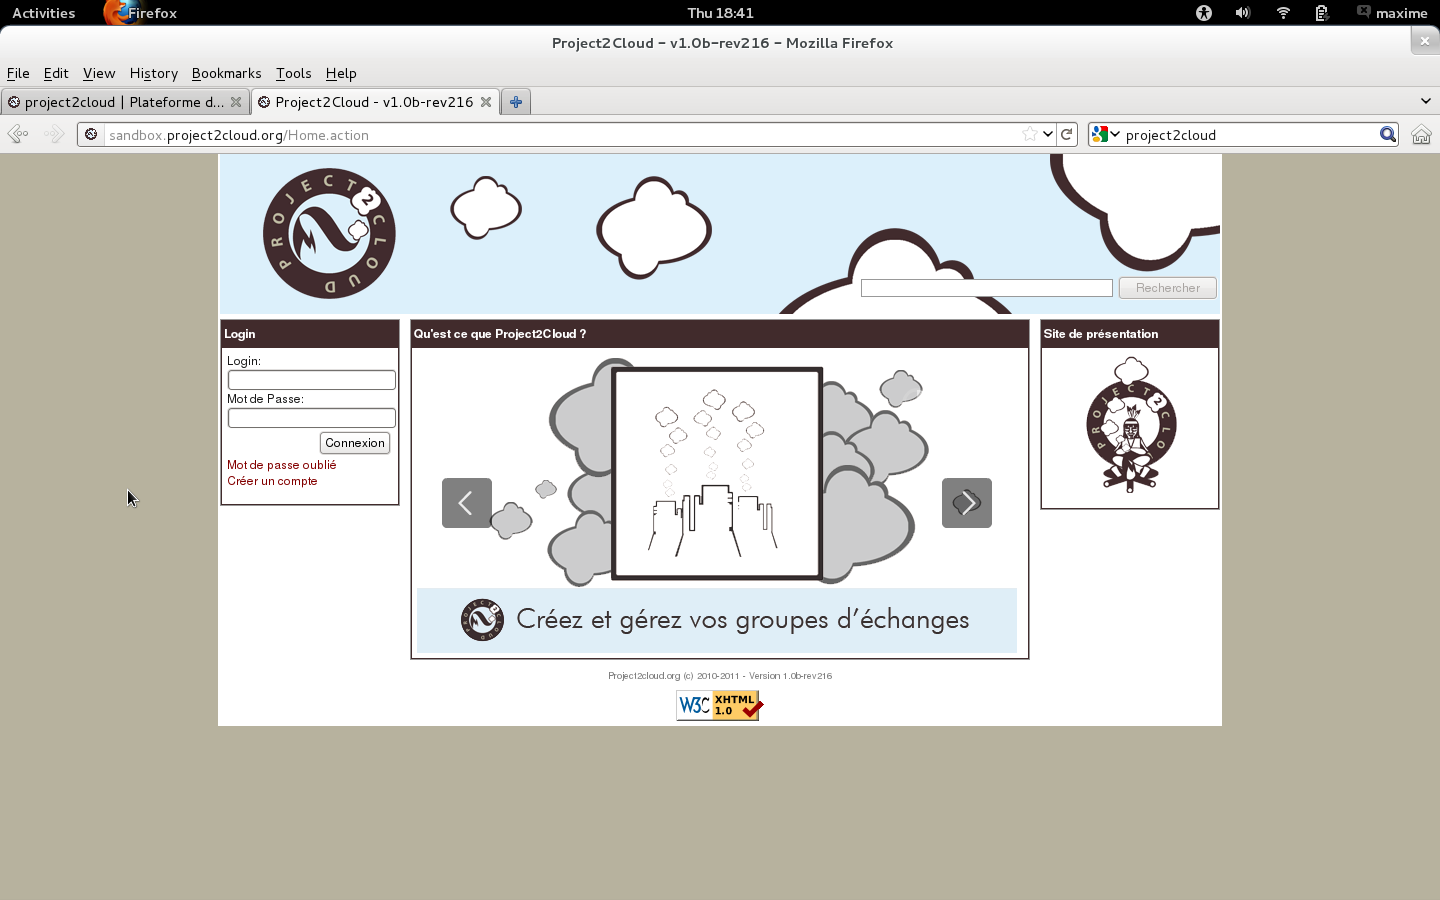
\includegraphics[width=350pt]{plateforme_d_essai}
					\caption{Plateforme Project2Cloud en béta-test.}			
				\end{center}
			\end{figure}
			
			\begin{figure}[H] 
				\begin{center}
					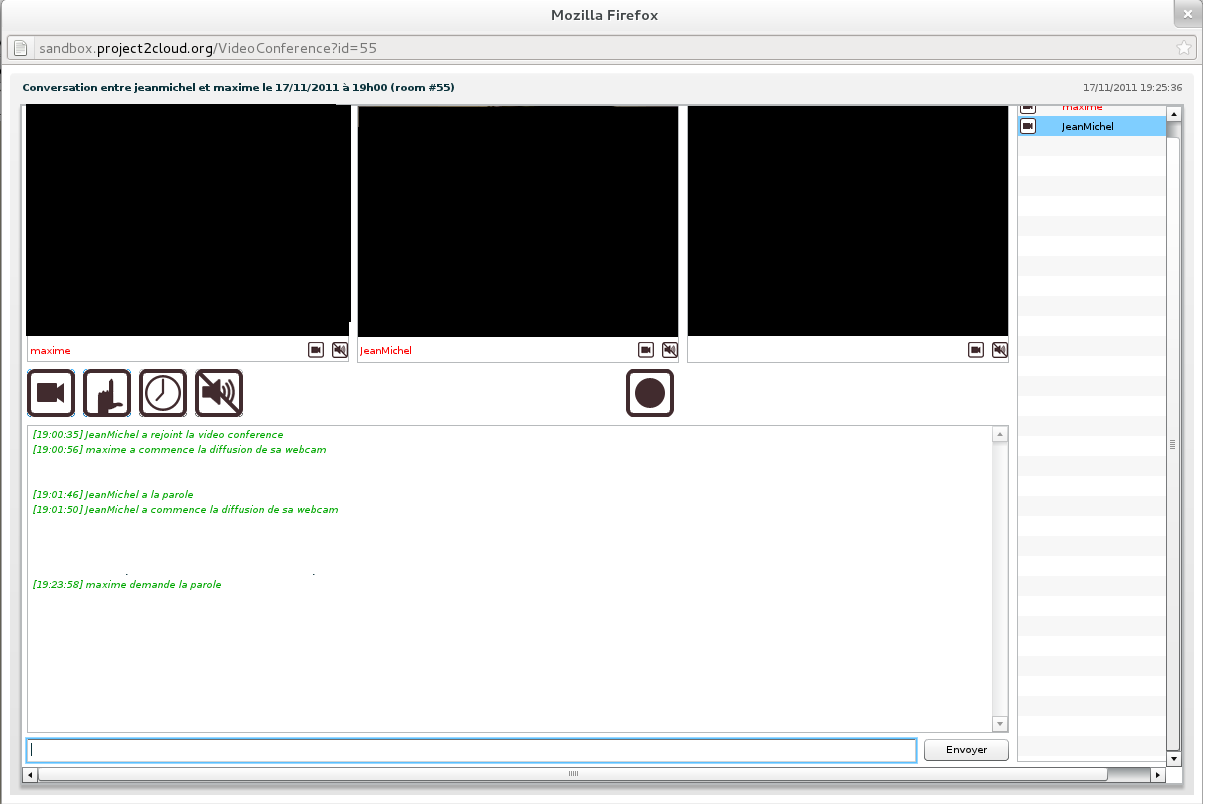
\includegraphics[width=350pt]{videoconf}
					\caption{Vidéo conférence avec Project2Cloud.}			
				\end{center}
			\end{figure}


	\section{Notre projet : Transcriptions audio vers texte pour des réunions enregistrées}
	Notre projet s'implantera directement dans la plate-forme P2C. Comme nous l'avons expliqué précédemment, P2C permettra aux utilisateurs de communiquer facilement grâce à un panel complet d'échanges vidéo, audio ou texte. Le but de notre projet est de faciliter l'indexation des conférences vidéos (c'est à dire de mieux séquencer temporellement les vidéos enregistrées). Pour cela, nous devrons ajouter une fonctionnalité supplémentaire : la transcription vocale des conversations. Concrètement, lors d'une conférence vidéo, les conversations des différents participants seront traduites en texte. Ce même texte sera enregistré sur un serveur. Le but est de permettre à un utilisateur de retrouver un mot ou un groupe de mot prononcé pendant une conférence, et de pouvoir visionner cette dernière à l'instant où le mot a été prononcé. On créé ainsi une "mémoire" des conférences, avec la possibilité de retrouver des informations très précises à des moments clés. 
	Notre projet est donc de convertir les conversations en texte, de les enregistrer, et de pouvoir indexer ces conversations à partir de mots clés. 

	\section{Analyse organisationnelle : dimension commerciale de notre projet}
	Notre projet vise donc à apporter une fonctionnalité supplémentaire à une plate-forme déjà existante. Cet aspect est intéressant, dans la mesure où des sites (ou des logiciels) proposant des conférences vidéos existent déjà (comme Skype par exemple). Project2Cloud propose de nouvelles options encore peu voire pas développée, dont notre projet de transcription vocale. On est donc en droit de se demander dans quelle mesure l'amélioration de la plateforme par notre projet peut-elle donner à l'entreprise l'opportunité d'étendre la distribution de son produit ?%
	
	
	%----------------------------------------------------- XIV. Conclusion -----------------------------------------------------%

		%--------------------------------------------------------- Conclusion ------------------------------------------------------%

	\addstarredpart{Conclusion}
	\chapter*{Conclusion}
	
	Cette conclusion doit faire la synthèse de l'état d'avancement du projet, de votre avis par rapport à cet état d'avancement, et décrire brièvement les prochaines étapes du projet.
	
	
	%--------------------------------------------------------- XV. Références ------------------------------------------------------%
	
	\addstarredpart{Références}
	\addstarredchapter{Bibliographie}
	\bibliographystyle{unsrt} % style de la biblio : comment on souhaite que les références s'affichent
	\bibliography{references} % nom de fichier des référénces : references.bib
	-
	
	
	
	
	
\end{document}